\documentclass[a4paper, onecolumn, 10pt]{article}

\usepackage[center,width=152mm,height=235mm]{crop}

\usepackage[english]{babel}
\usepackage[latin1]{inputenc}
\usepackage[T1]{fontenc}
\usepackage{selinput}
\SelectInputMappings{%
  aacute={á},
  ntilde={ñ},
  Euro={€}
}

\usepackage{float} % For controlling figure positions
\usepackage{amsthm, amsmath, amsfonts, amssymb}
\usepackage{fancybox}
\usepackage{color}
\usepackage{cite}
\usepackage{url}

\usepackage{tikz}
\usetikzlibrary{shapes,arrows}
% Define block styles
\tikzstyle{state} = [rectangle, draw, fill=blue!20, 
    text width=5em, text centered, rounded corners, minimum height=4em]
\tikzstyle{line} = [draw, -latex']
\tikzstyle{source} = [draw, ellipse,fill=red!20, node distance=3cm,
    minimum height=2em]

\usepackage{graphicx}
\graphicspath{ {../../img/} }

\usepackage[draft, colorinlistoftodos]{todonotes} % Use disable instead of draft to hide todo notes

\usepackage[switch]{lineno} % Activate using \linenumbers

% Simulation parameters
%\newcommand{\numReps}{200} % Number of repetitions
%\newcommand{\stabilTime}{2000} % Stabilization time
%\newcommand{\simTime}{5000} % Simulation time
%\newcommand{\numEpsilons}{23} % Number of epsilons to be tried
%\newcommand{\numExps}{4600} % Total number of experiments \numReps * \numEpsilons

\usepackage{authblk}
\title{Notes}
\author[1]{Pablo Rodríguez-Sánchez \thanks{\texttt{pablo.rodriguezsanchez@wur.nl}}}
%\author[1]{Egbert H. van Nes \thanks{\texttt{egbert.vannes@wur.nl}}}
%\author[1]{Marten Scheffer \thanks{\texttt{marten.scheffer@wur.nl}}}

\affil[1]{Department of Aquatic Ecology, Wageningen University, The Netherlands}

%% Override to comply with amnat guidelines
%\linespread{1.7}
%\linenumbers
%\modulolinenumbers[2]

\begin{document}

\maketitle

\clearpage

\section{Dissecting the Phillips Robinson model}
\label{sec:Dissecting}
In reference \cite{Phillips2007} a sleep-wake model is described with detail. The model uses three state variables (see table \ref{tab:StateVariables}).

\begin{table}[h]
	\begin{tabular}{|c|c|c|}
		\hline 
		State variable & Physiological interpetation & Informal interpretation \\ 
		\hline 
		$V_v$ & Activity of the VLPO & Stay asleep system \\ 
		\hline 
		$V_m$ & Activity of the MA & Stay awake system \\ 
		\hline 
		$H$ & Homeostatic pressure & Somnogen level \\ 
		\hline 
\end{tabular}
\caption{State variables in the Phillips Robinson model}
\label{tab:StateVariables}
\end{table}

The dynamics are described by equation \ref{eq:PhilRobModel}, where $S$ is a sigmoidal saturation function given by equation \ref{eq:Saturation}, and $C(t)$ (see equation \ref{eq:Drive}) is the day/night external forcing. The interactions in the dynamical equations are summarized in figure \ref{fig:PhilRobModel}.

Equation \ref{eq:PhilRobModel} has been carefully structured. The left hand side alone represents an uncoupled exponential decay for each of the three state variables. The matrix product term in the right hand side represents the system's coupling. The vector addition in the right hand side accounts for the sources of the system, being one of them time-dependent.

\begin{equation}
\label{eq:PhilRobModel}
\left[
\begin{array}{c}
\tau_v \dot V_v + V_v \\ 
\tau_m \dot V_m + V_m \\ 
\chi \dot H + H
\end{array}
\right]
=
\left[
\begin{array}{ccc}
0 & -\nu_{vm} & \nu_{vh} \\ 
-\nu_{mv} & 0 & 0 \\ 
0 & \mu & 0
\end{array}
\right] 
\left[
\begin{array}{c}
S(V_v) \\ 
S(V_m) \\ 
H
\end{array}
\right]
+
\left[
\begin{array}{c}
-\nu_{vc} C(t) \\ 
\nu_{ma} S(V_{a0}) \\ 
0
\end{array}
\right]
\end{equation}

\begin{equation}
\label{eq:Saturation}
S(V) = \frac{Q_{max}}{1 + e^{-\frac{V-\theta}{\sigma}}}
\end{equation}

\begin{equation}
\label{eq:Drive}
C(t) = \frac{1}{2} \left( 1 + cos(\omega t + \alpha) \right)
\end{equation}

\begin{figure}[h]
\label{fig:PhilRobModel}
\begin{center}
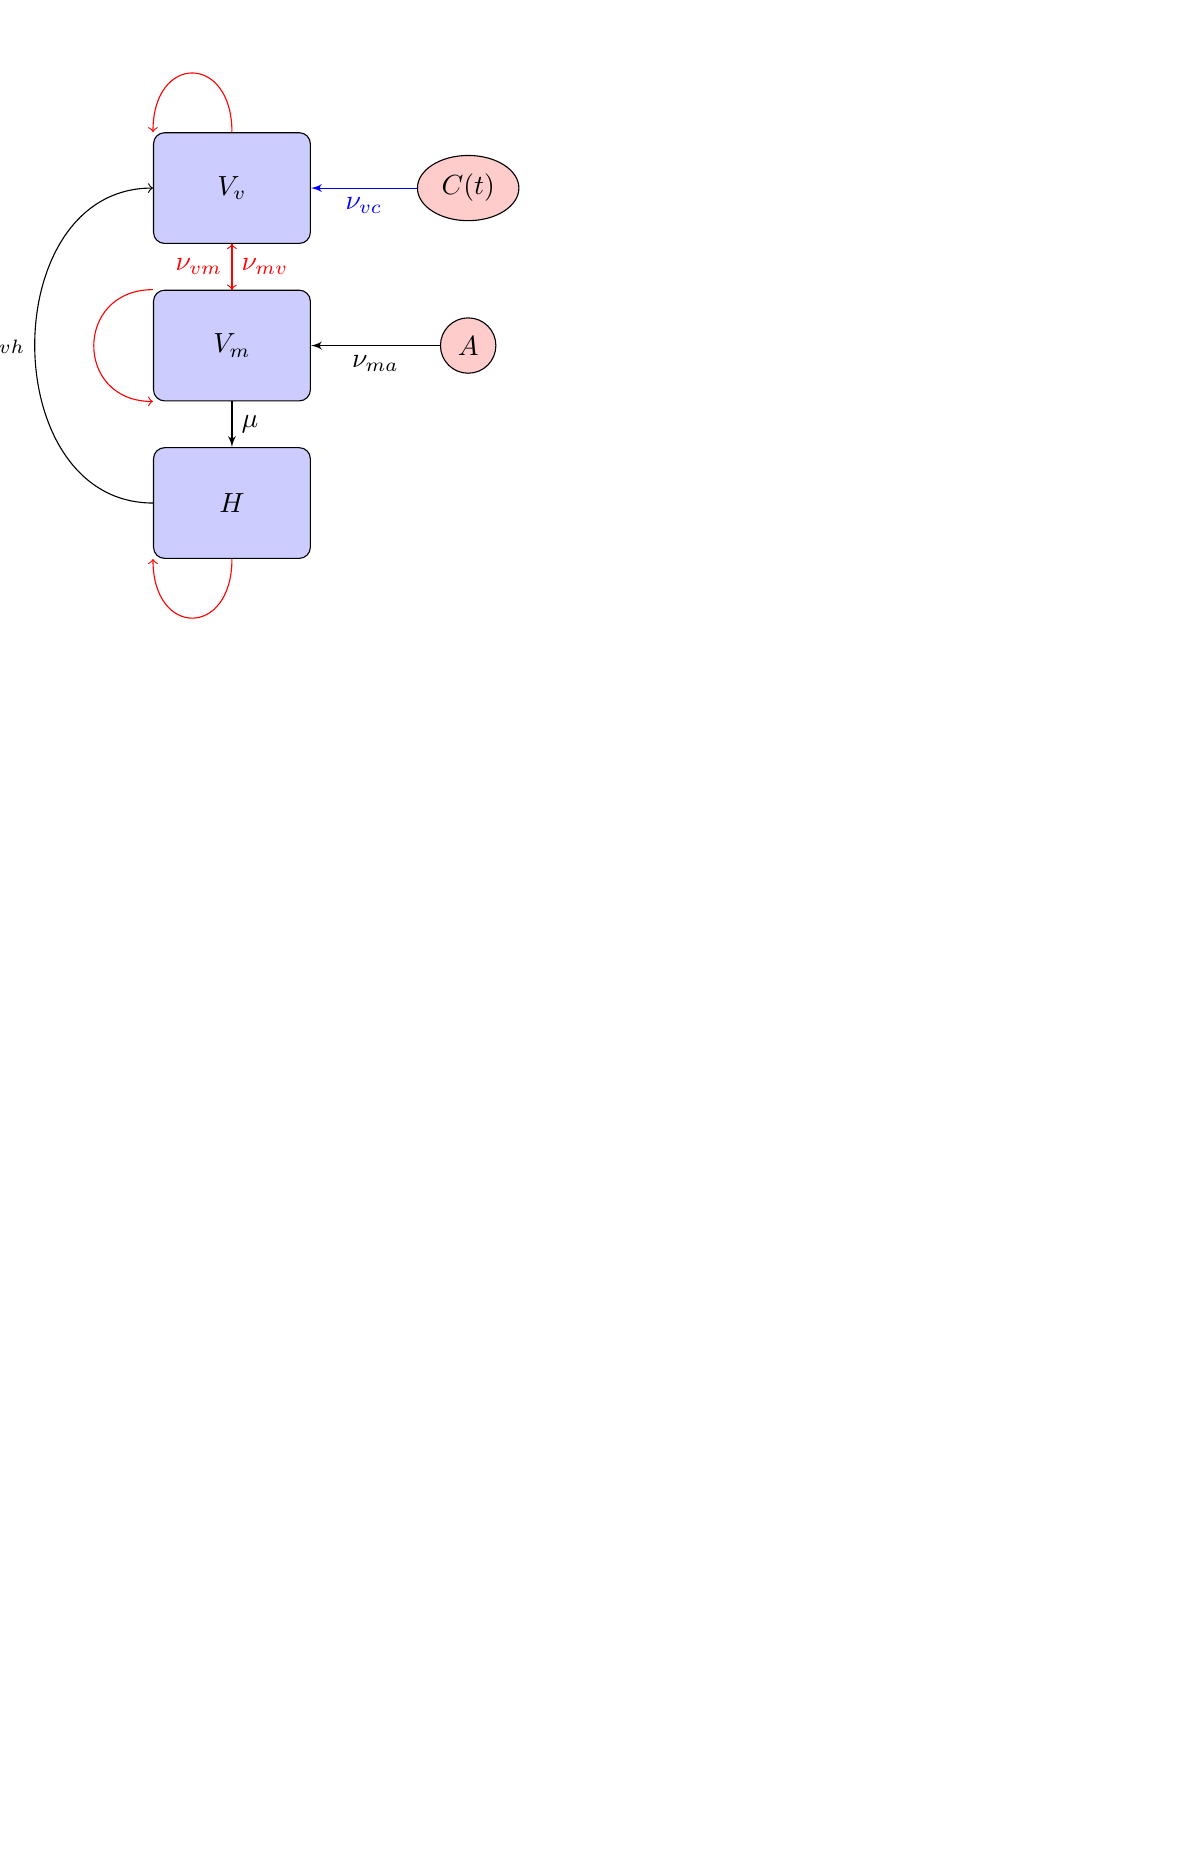
\begin{tikzpicture}[node distance = 2cm, auto]
    % Place nodes
    % States
    \node [state] (Vv) {$V_v$};
    \node [state, below of=Vv] (Vm) {$V_m$};
    \node [state, below of=Vm] (H) {$H$};
    
    % Sources
    \node [source, right of=Vv] (C) {$C(t)$};
    \node [source, right of=Vm] (A) {$A$};
    
    % Draw edges
    % Sources
    \path [blue, line] (C) -> node{$\nu_{vc}$} (Vv);
    \path [line] (A) -> node{$\nu_{ma}$} (Vm);
    
    % Coupling
    \path [line] (Vm) -> node{$\mu$} (H);
    \draw[red, ->] (Vv) -- node[midway, right] {$\nu_{mv}$} (Vm);
    \draw[red, ->] (Vm) -- node[midway, left] {$\nu_{vm}$} (Vv);
    \draw[->] (H.west) .. controls +(left:20mm) and +(left:20mm) .. node{$\nu_{vh}$} (Vv.west);
    
    % Decay
    \draw[red, ->] (Vv.north) .. controls +(up:10mm) and +(up:10mm) .. (Vv.north west);
    \draw[red, ->] (Vm.north west) .. controls +(left:10mm) and +(left:10mm) .. (Vm.south west);
    \draw[red, ->] (H.south) .. controls +(down:10mm) and +(down:10mm) .. (H.south west);

\end{tikzpicture}
\end{center}
\caption{Schematic summary of the dynamics. The blue nodes represent the system's states ($V_v$ the activity of the ventrolateral preoptic area, $V_m$ the activity of the mono aminergic group and $H$ the homeostatic pressure). The red nodes represent the external sources ($C(t)$, the astronomical light/dark forcing, and $A$, the acetylcholine group constant influence). The positive effects are coded as black arrows. Negative ones as red arrows. Blue arrows represent oscillating effects.}
\end{figure}

The time series typically oscillate with a daily cycle (see figure \ref{fig:Typical}).

\begin{figure}[h]
	\begin{center}
		\includegraphics[width=1\columnwidth]{typical.png}
	\end{center}
	\caption{}
	\label{fig:Typical}
\end{figure}

\clearpage

In order to shed some light into the behaviour of the model, we'll study subsets of it by removing some terms in the main equation \ref{eq:PhilRobModel}.

\subsection{No sources nor coupling}
The dynamics of the three state variables, in the absence of coupling and sources, are those of an uncoupled exponential decay (see figure \ref{fig:DeadPhilRobModel} and equation \ref{eq:DeadPhilRobModel}).

\begin{equation}
\label{eq:DeadPhilRobModel}
\left[
\begin{array}{c}
\tau_v \dot V_v + V_v \\ 
\tau_m \dot V_m + V_m \\ 
\chi \dot H + H
\end{array}
\right]
=
\left[
\begin{array}{c}
0 \\ 
0 \\ 
0
\end{array}
\right]
\end{equation}

\begin{figure}[h]
\begin{center}
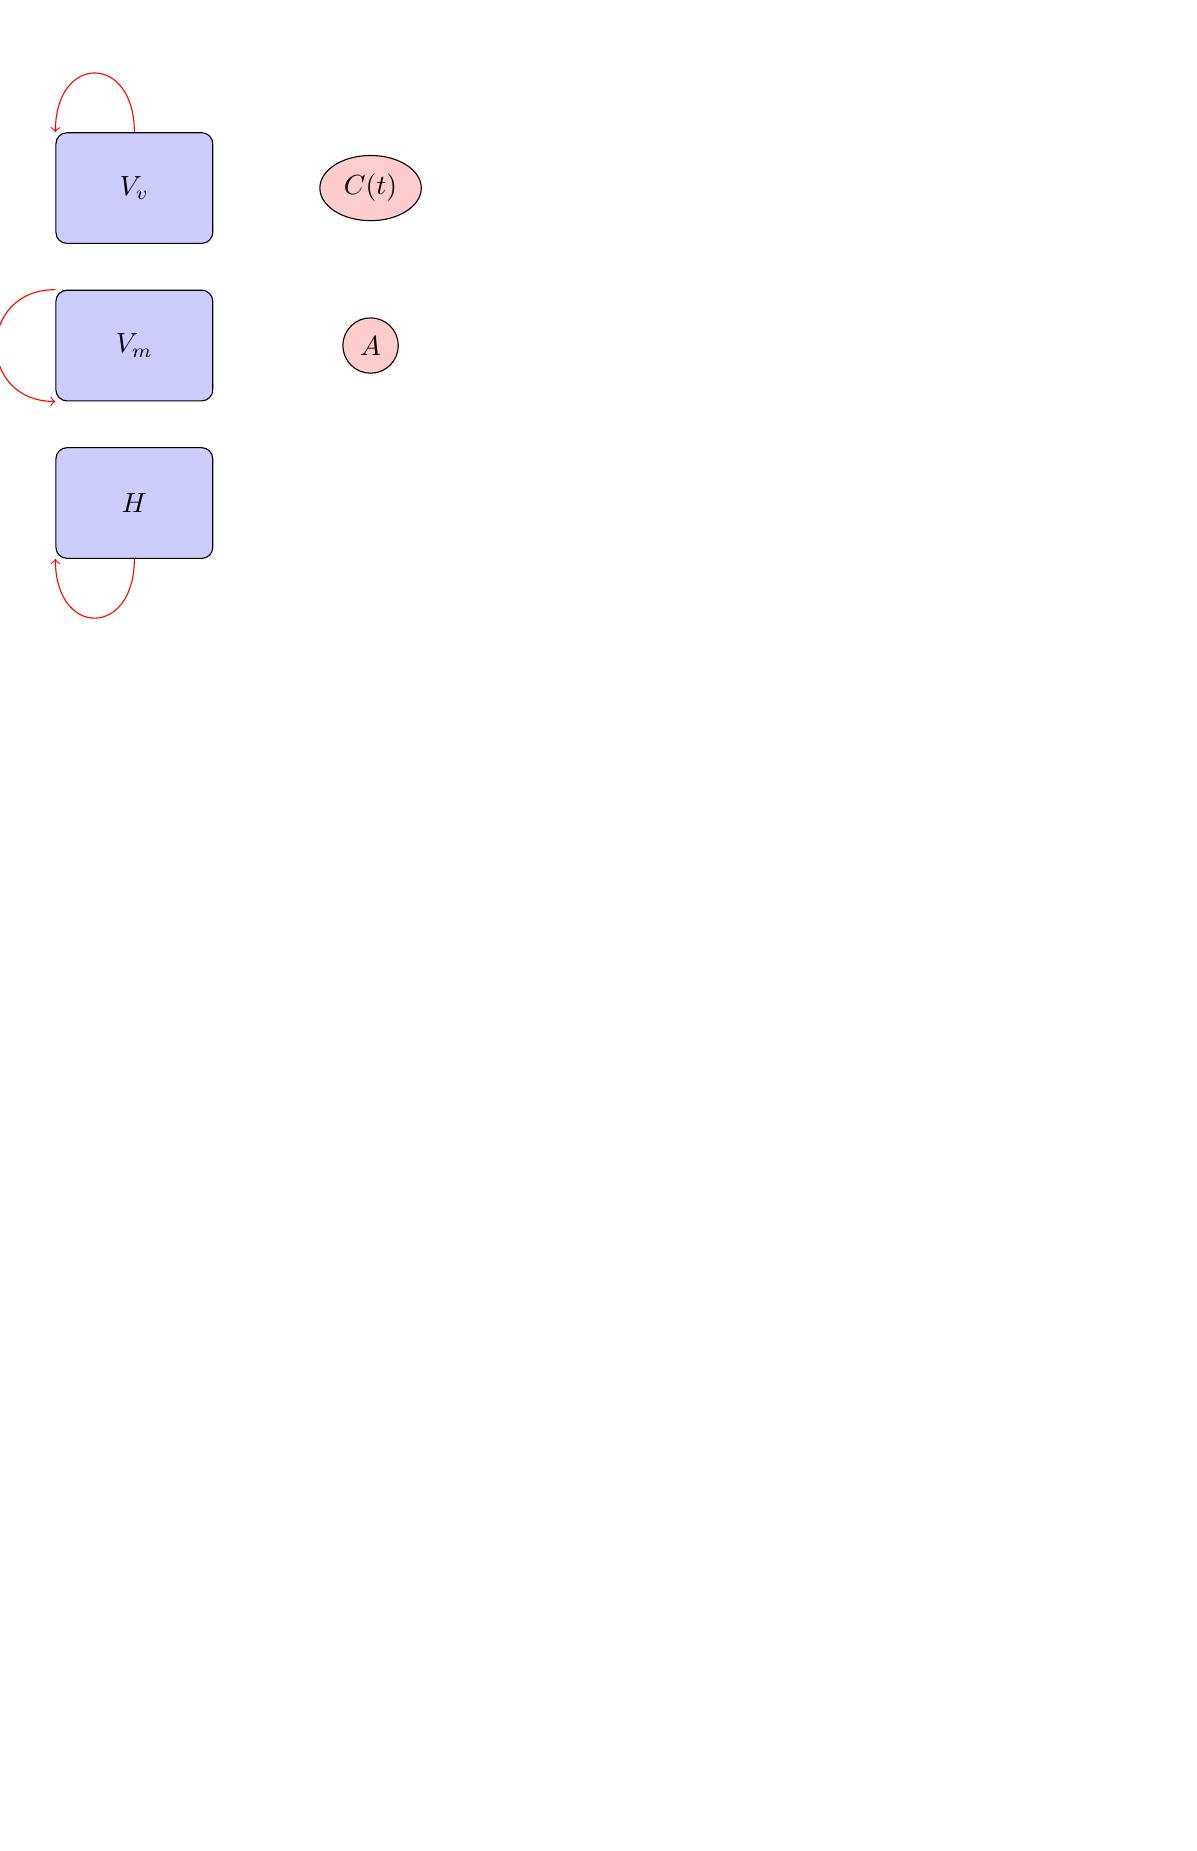
\begin{tikzpicture}[node distance = 2cm, auto]
    % Place nodes
    % States
    \node [state] (Vv) {$V_v$};
    \node [state, below of=Vv] (Vm) {$V_m$};
    \node [state, below of=Vm] (H) {$H$};
    
    % Sources
    \node [source, right of=Vv] (C) {$C(t)$};
    \node [source, right of=Vm] (A) {$A$};
    
    % Draw edges
    % Decay
    \draw[red, ->] (Vv.north) .. controls +(up:10mm) and +(up:10mm) .. (Vv.north west);
    \draw[red, ->] (Vm.north west) .. controls +(left:10mm) and +(left:10mm) .. (Vm.south west);
    \draw[red, ->] (H.south) .. controls +(down:10mm) and +(down:10mm) .. (H.south west);

\end{tikzpicture}
\end{center}
\caption{After removing all the terms in the right hand side of equation \ref{eq:PhilRobModel}, the remaining system can be schematized like this.}
\label{fig:DeadPhilRobModel}
\end{figure}

All the time series just decay to zero (see figure \ref{fig:Decay}).

\begin{figure}[h]
	\begin{center}
		\includegraphics[width=1\columnwidth]{decay.png}
	\end{center}
	\caption{}
	\label{fig:Decay}
\end{figure}

\clearpage
\subsection{Sources and no coupling}
If the external sources are switched on, the behaviour of $V_m$ and $H$ is still exponential decay. $V_v$ oscillates synchronously with the frequency of the external time dependent influence $C(t)$. The system is still uncoupled (see figure \ref{fig:OnlySourcesPhilRobModel} and equation \ref{eq:OnlySourcesPhilRobModel}).

\begin{equation}
\label{eq:OnlySourcesPhilRobModel}
\left[
\begin{array}{c}
\tau_v \dot V_v + V_v \\ 
\tau_m \dot V_m + V_m \\ 
\chi \dot H + H
\end{array}
\right]
=
\left[
\begin{array}{c}
-\nu_{vc} C(t) \\ 
\nu_{ma} S(V_{a0}) \\ 
0
\end{array}
\right]
\end{equation}


\begin{figure}[h]
\label{fig:OnlySourcesPhilRobModel}
\begin{center}
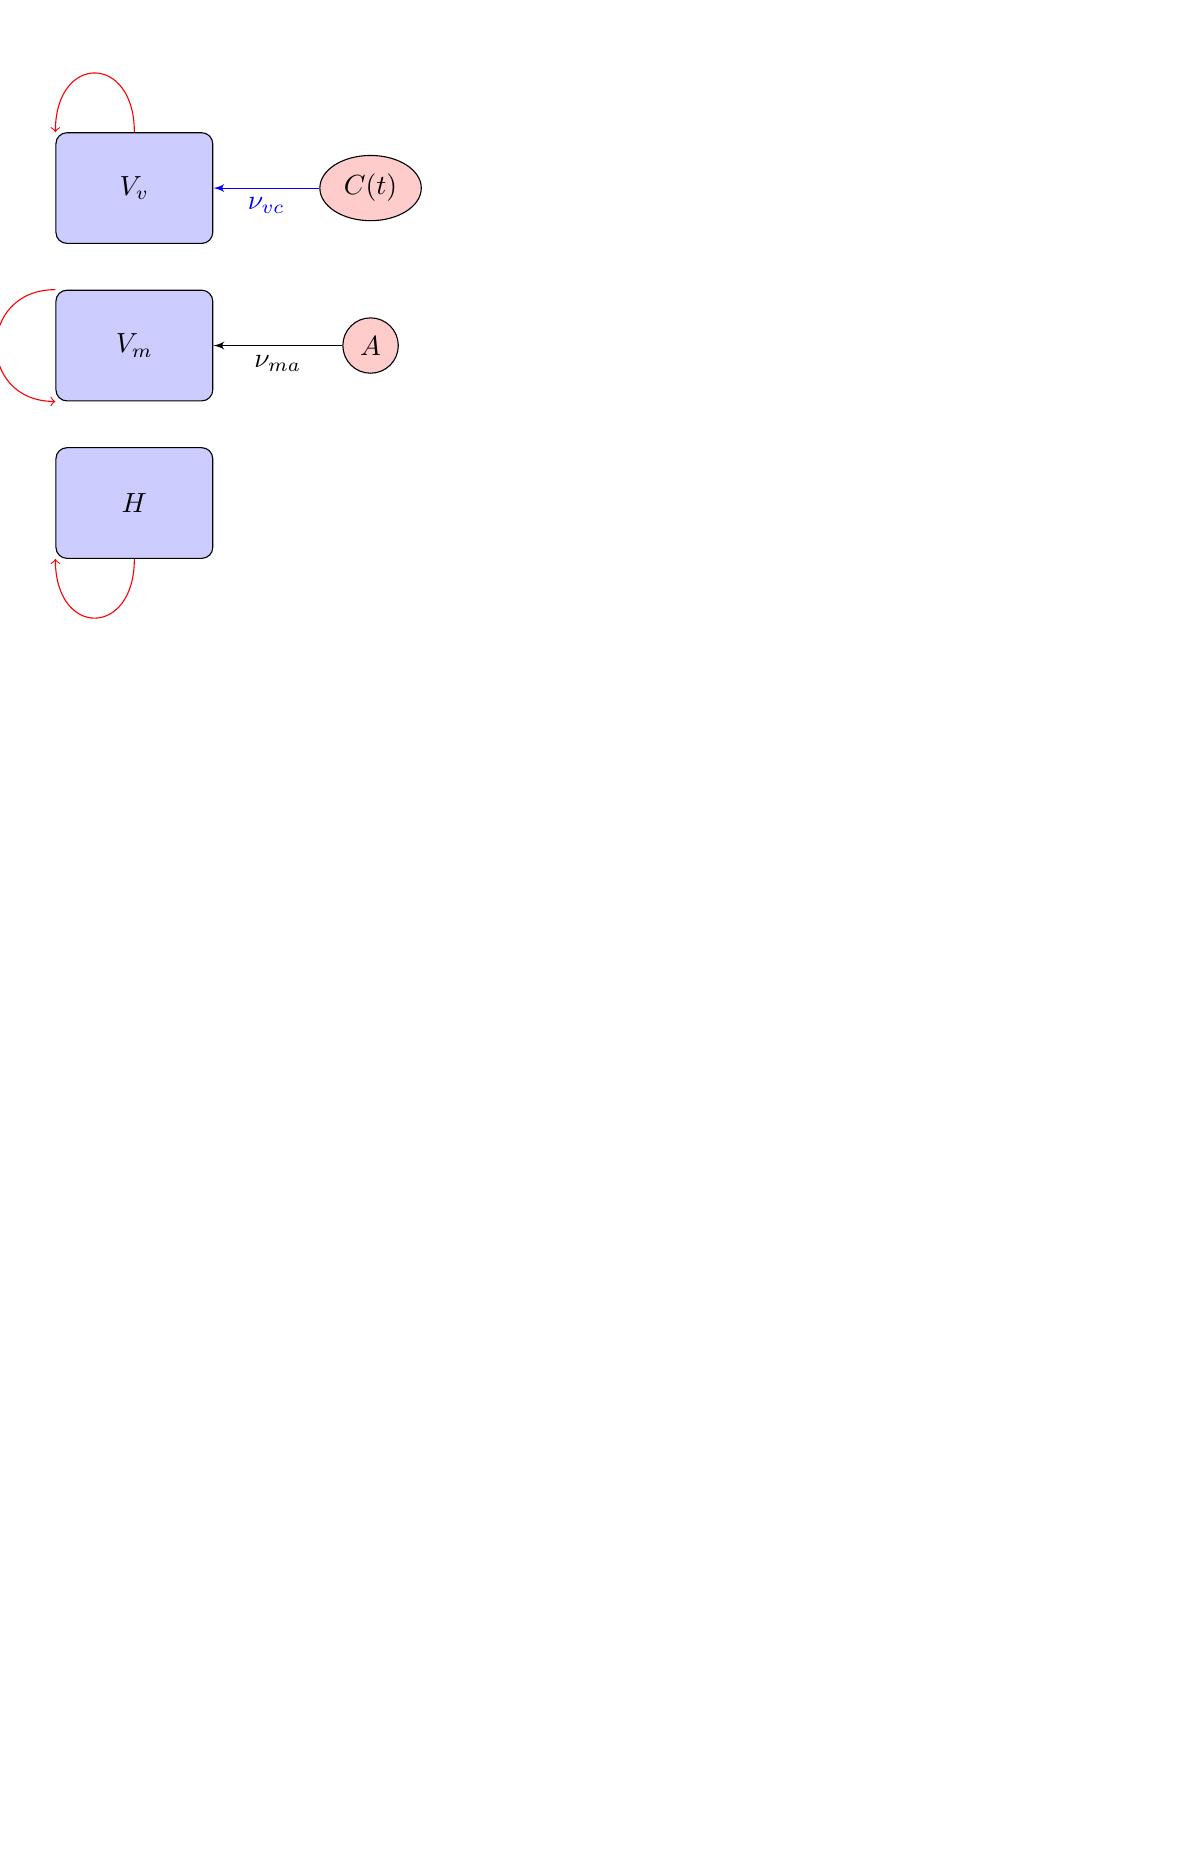
\begin{tikzpicture}[node distance = 2cm, auto]
    % Place nodes
    \node [state] (Vv) {$V_v$};
    \node [state, below of=Vv] (Vm) {$V_m$};
    \node [state, below of=Vm] (H) {$H$};
    
    \node [source, right of=Vv] (C) {$C(t)$};
    \node [source, right of=Vm] (A) {$A$};
    
    % Draw edges
    % Sources
    \path [blue, line] (C) -> node{$\nu_{vc}$} (Vv);
    \path [line] (A) -> node{$\nu_{ma}$} (Vm);
    
    % Decay
    \draw[red, ->] (Vv.north) .. controls +(up:10mm) and +(up:10mm) .. (Vv.north west);
    \draw[red, ->] (Vm.north west) .. controls +(left:10mm) and +(left:10mm) .. (Vm.south west);
    \draw[red, ->] (H.south) .. controls +(down:10mm) and +(down:10mm) .. (H.south west);

\end{tikzpicture}
\end{center}
\caption{Summary of the dynamics}
\end{figure}

The time series of $V_m$ and $H$ decay exponentially. $V_v$ oscillates with the frequency of the external forcing $C(t)$ (see figure \ref{fig:Uncoupled}).

\begin{figure}[h]
	\begin{center}
		\includegraphics[width=1\columnwidth]{uncoupled.png}
	\end{center}
	\caption{}
	\label{fig:Uncoupled}
\end{figure}

\clearpage
\subsection{Autonomous system}
Interestingly enough, making $\nu_{vc} = 0$ (and thus removing completely the astronomical light/dark influence) the system reaches a cyclic attractor, whose period is roughly $8$ hours (see equation \ref{eq:AutoPhilRobModel} and figure \ref{fig:AutoPhilRobModel}).

\begin{equation}
\label{eq:AutoPhilRobModel}
\left[
\begin{array}{c}
\tau_v \dot V_v + V_v \\ 
\tau_m \dot V_m + V_m \\ 
\chi \dot H + H
\end{array}
\right]
=
\left[
\begin{array}{ccc}
0 & -\nu_{vm} & \nu_{vh} \\ 
-\nu_{mv} & 0 & 0 \\ 
0 & \mu & 0
\end{array}
\right] 
\left[
\begin{array}{c}
S(V_v) \\ 
S(V_m) \\ 
H
\end{array}
\right]
+
\left[
\begin{array}{c}
0 \\ 
\nu_{ma} S(V_{a0}) \\ 
0
\end{array}
\right]
\end{equation}

\begin{figure}[h]
\label{fig:AutoPhilRobModel}
\begin{center}
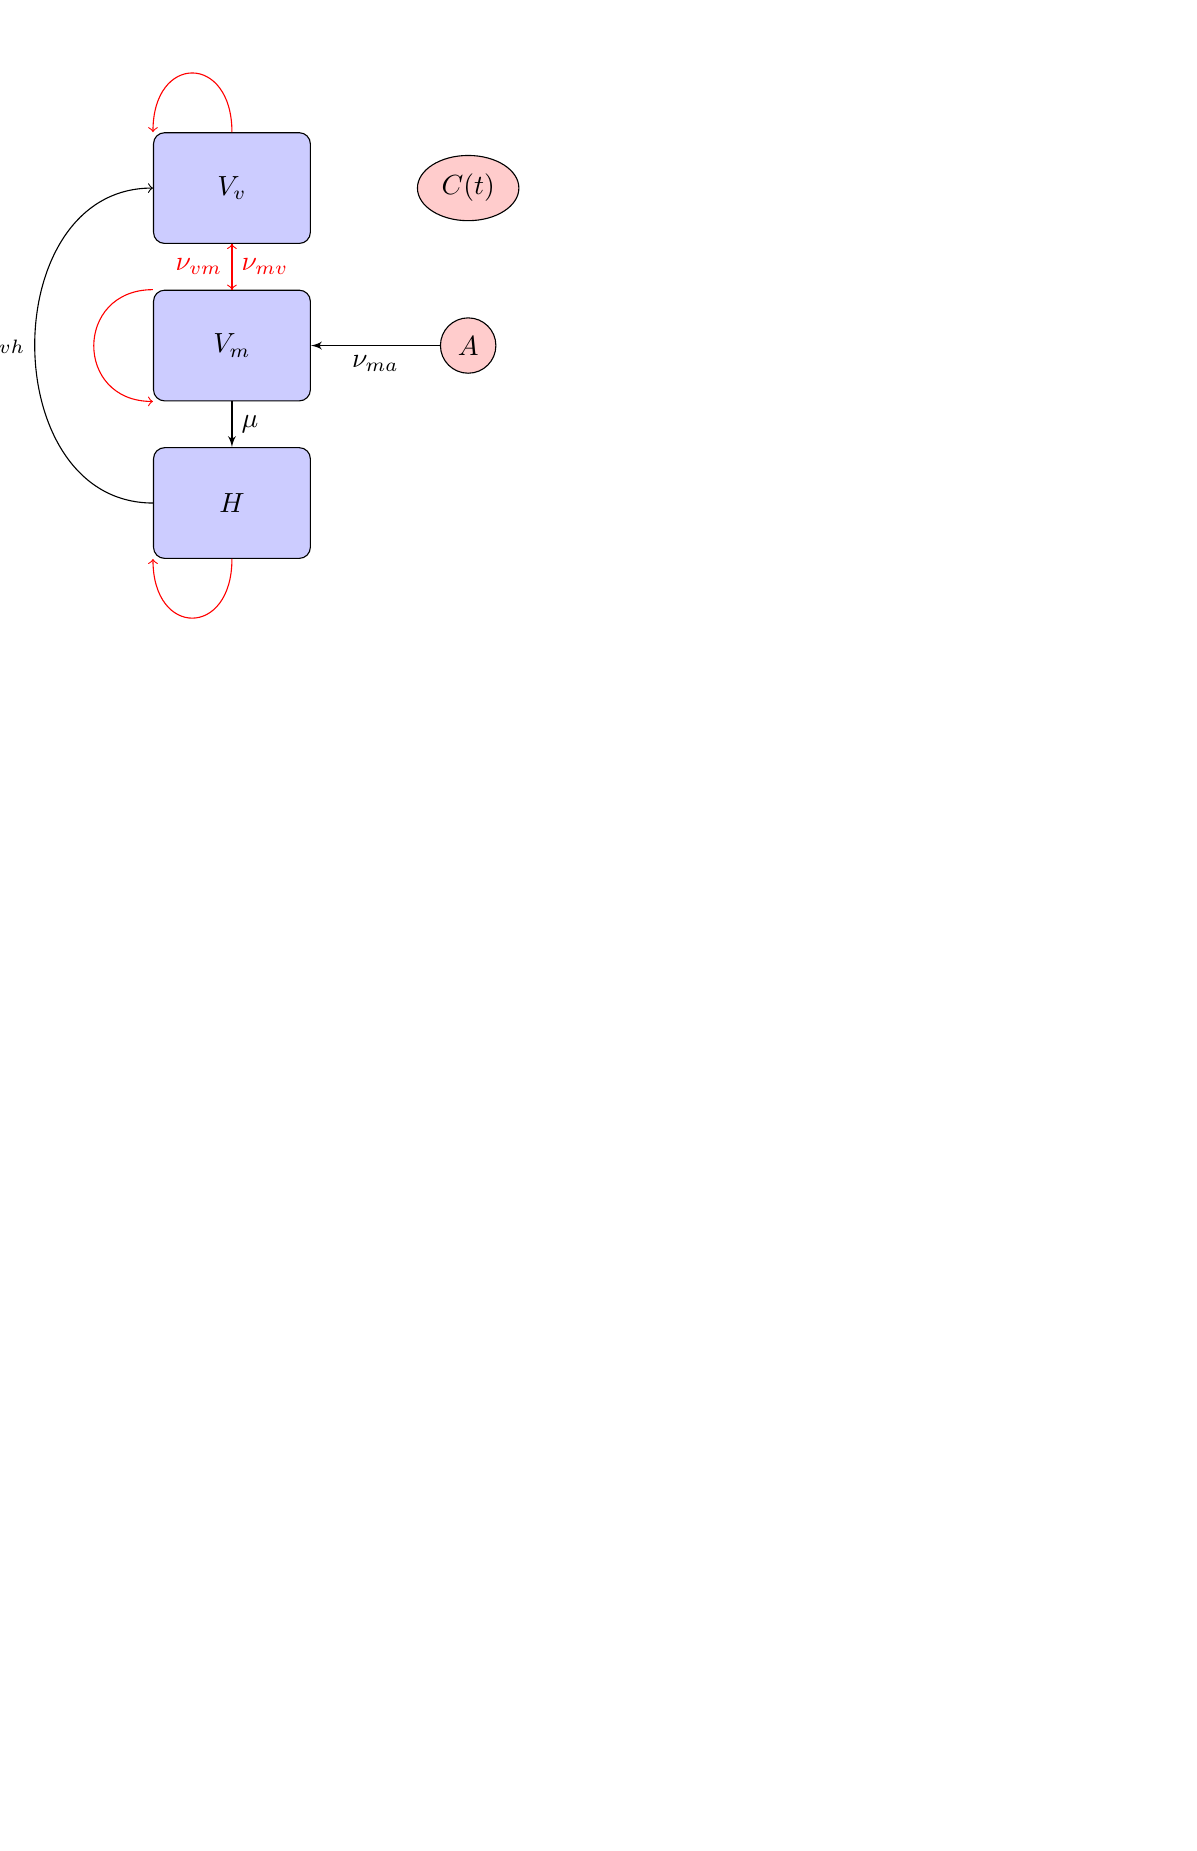
\begin{tikzpicture}[node distance = 2cm, auto]
    % Place nodes
    % States
    \node [state] (Vv) {$V_v$};
    \node [state, below of=Vv] (Vm) {$V_m$};
    \node [state, below of=Vm] (H) {$H$};
    
    % Sources
    \node [source, right of=Vv] (C) {$C(t)$};
    \node [source, right of=Vm] (A) {$A$};
    
    % Draw edges
    % Sources
    \path [line] (A) -> node{$\nu_{ma}$} (Vm);
    
    % Coupling
    \path [line] (Vm) -> node{$\mu$} (H);
    \draw[red, ->] (Vv) -- node[midway, right] {$\nu_{mv}$} (Vm);
    \draw[red, ->] (Vm) -- node[midway, left] {$\nu_{vm}$} (Vv);
    \draw[->] (H.west) .. controls +(left:20mm) and +(left:20mm) .. node{$\nu_{vh}$} (Vv.west);
    
    % Decay
    \draw[red, ->] (Vv.north) .. controls +(up:10mm) and +(up:10mm) .. (Vv.north west);
    \draw[red, ->] (Vm.north west) .. controls +(left:10mm) and +(left:10mm) .. (Vm.south west);
    \draw[red, ->] (H.south) .. controls +(down:10mm) and +(down:10mm) .. (H.south west);

\end{tikzpicture}
\end{center}
\caption{In the absence of influence from the external, astronomical light/dark cycle, our system is still capable of oscillating.}
\end{figure}

\begin{figure}[h]
	\begin{center}
		\includegraphics[width=1\columnwidth]{auto.png}
	\end{center}
	\caption{In the absence of external periodic forcing, the system oscillates with an internal, approximate frequency of 8 h}
	\label{fig:Auto}
\end{figure}

%% Bibliography
\clearpage
\bibliography{../bib/library}
\bibliographystyle{vancouver}

\end{document}
